
The generation of electrical signals within a phantom head is the core mechanism enabling the controlled validation of new electrode and instrumentation designs~\cite{9475461}. Unlike experiments conducted on human subjects where the recorded signal is intrinsically unknown, phantoms allow a pre-recorded electrophysiology signal or a synthetically created signal to be played out, providing a known signal for the test system to collect and compare against~\cite{Owda2020}. This is usually achieved by injecting precisely controlled currents or voltages into the phantom's conductive medium via a set of internal drive electrodes~\cite{akor-2025}.

Phantom designs then consist of primarily three components: the electrode array that injects the signal into the phantom, the electrode driver that allows the independent control of each electrode, and the phantom head itself that contains said electrode array~\cite{LEAHY1998159}.

As phantom head design and composition where already covered in subsubsection~\ref{subsec:phantom_designs} and subsubsection~\ref{subsec:phantom_materials} respectively, this subsection focuses on the signal generation module (electrode array and driver) and the key characteristics of the generated signals.

\paragraph{Signal Requirements}

Phantom heads are designed to mimic the frequency spectrum of human brain activity, which is characterized by a wide range of frequencies. Specific frequency bands used in phantom validation include:

\begin{itemize}
    \item Standard bands: Phantoms are often tested against standard clinical bands, such as Delta (0.5{-}4 Hz), Theta (4{-}7 Hz), Alpha (8{-}12 Hz) and Beta (13{-}30 Hz)~\cite{akor-2025}.
    \item Higher frequencies: Gamma, 30{-}80 Hz and higher, are more difficult to study in the human body as they are heavily attenuated by the skull and scalp layers, and obfuscated by muscular and ocular artifacts~\cite{FREEMAN20031053}. Head phantom validation often involves ensuring that the components accurately mimic these behaviours~\cite{9475461}.
\end{itemize}

The amplitude of the EEG under physiological conditions ranges from 15 to 150 \( \mu\text{V} \)~\cite{Naydenov2022}. However, the internal generators (electrodes) must drive significantly higher voltages to account for the attenuation caused by volume conduction through the phantom material~\cite{LEAHY1998159}. The electronics must provide a wide dynamic range, capable of generating signals that result in low surface potentials to reduce noise~\cite{Morsalin2020}.

\paragraph{Electrode Driver}

The electrode driver acts as the interface between the digital simulation software (usually on a PC) and the physical phantom, generating complex, arbitrary waveforms used to mimic neural activity~\cite{LEAHY1998159}.

Controlling the driver means knowing the exact location, orientation, amplitude, and timing of the source: the ``ground truth'' data~\cite{LEAHY1998159}. This known signal is crucial for validating the performance of EEG electrodes and acquisition systems, as it allows for objective comparisons between the generated signal and the recorded data.~\cite{Audette2020}

\paragraph{Electrode Construction}
The driver controls the known electrical signals that are injected into physical electrodes embedded in the phantom head. These electrodes can be constructed in various ways depending on the design requirements of the phantom:

\begin{itemize}
    \item The most common are dipoles constructed from semi-rigid coaxial cables, where the inner conductor and the outer shield are exposed at the tip (with a gap of roughly 0.5 mm to 2 mm) to form the two poles of the dipole (see Figure~\ref{fig:dipole_leahy}). This design is favored because the semi-rigid nature of the cable allows for precise positioning and bending to specific orientations within the phantom volume~\cite{LEAHY1998159}.
    \item For high-fidelity phantoms, platinum electrodes are used as they are chemically inert and resistant to corrosion, which is a major concern in saline environments~\cite{Machts2019}.
    \item For lower-cost phantoms, standard 3.5 mm TRS audio jacks are used. While less electrochemically stable than platinum, they are readily available and provide a standardized connection interface.~\cite{Downey2023}
\end{itemize}

\begin{figure}
\centering
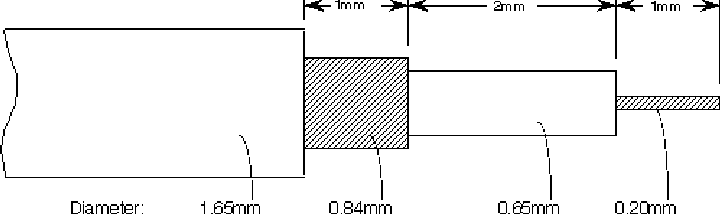
\includegraphics[width=0.5\textwidth]{../../02_Images/leahy_dipole.png}
\caption[Coaxial cable dipole electrode]{Coaxial cable dipole used in~\cite{LEAHY1998159}.}
\label{fig:dipole_leahy}
\end{figure}

\paragraph{Electronic module architecture}

The choice of architecture dictates the fidelity, bandwidth, and flexibility of the phantom. Some common architectures include:

\begin{itemize}
    \item Computer audio interface: frequently used for this task due to their high resolution (typically 24-bit), excellent signal-to-noise ratio (>100 dB), and low cost~\cite{Collier2012}. The downside is that they tether the phantom to a computer, introducing ground loops and mains noise unless USB isolators are used~\cite{LEAHY1998159}.
    \item Microcontroller-based architecture: for portable, battery-powered phantoms. A usual choice is the Teensy 3.2 that features a built-in 12-bit digital-to-analog converter (DAC)~\cite{PJRC_Teensy}. While having lower resolution than audio interfaces, 12 bits provides sufficient dynamic range for many verification tasks, especially when the signal is generated at a higher amplitude and then attenuated analogically~\cite{LEAHY1998159}.
\end{itemize}

\paragraph{Wireless Protocols}

\nota{Me gustaría añadir una sección sobre protocolos wireless para la transmisión de datos y control del phantom, pero no encontré mucho todavía. Ver cómo esto afecta a la señal que se transmite. Ver Audette2020}
